\documentclass[../main.tex]{subfiles}
\graphicspath{{\subfix{../figures/}}}
\begin{document}

The theory of quantum mechanics developed in the last century has been proved to be extremely successful in describing nature at the small scale. Typical systems treated by standard quantum mechanics are nuclei, atoms, and other systems which can be assumed to be isolated from the environment. In such systems, the Hamiltonian is postulated to be Hermitian, guaranteeing that energies are real-valued and that the wave function is contained in the system throughout the evolution (source, sakurai?). However, for many physical setups we cannot assume the system to be isolated and we must consider the crosstalk between the system and its surroundings. One way to handle such open systems is to loosen the requirement of the Hermiticity of the Hamiltonian. The resulting field of non-Hermitian quantum physics has successfully been describing systems in nuclear, atomic and optical physics in recent decades~\cite{nonHermrev}. One property of particular interest in non-Hermitian operators is the possibility of exceptional points (EPs). These correspond to points in parameter space where two or more eigenvalues and their corresponding eigenvectors of the operator simultaneously coalesce. Exceptional points have been proposed to have several useful technological applications, and along with the optical microring experiments in 2017, EP sensors successfully increased the sensitivity of current and nano-particle detection~\cite{microring1, microring2}.

A different framework which treats open systems is quantum master equations, where the dynamics of the system is captured by the Liouvillian superoperator. Similarly to the Hamiltonian in non-Hermitian physics, the Liouvillian is non-Hermitian due to the coupling to the environment. This brings the possibility of EPs also in the Liouvillian superoperator. EPs in Liouvillian physics have been of particular theoretical interest recently, and are proposed to have important applications in control and sensing technologies. Two recent examples include Ref.~\cite{thermal}, where critical decay towards the steady state in a quantum thermal machine was found at the EP; and in Ref.~\cite{steering} where an EP corresponded to optimal steering toward a target quantum state. 

An application of particular interest for quantum master equations and Liouvillian physics is electron transport in systems of quantum dots connected to metallic leads~\cite{qdottrans}. A quantum dot (QD) is a fabricated semiconductor structure containing a small number of electrons and is typically in the order of 100 nanometres in size~\cite{qdotmarcus}. The size of the dot needs to be small in comparison to the thermal wavelength of the electrons, which is why experiments are generally realized at temperatures close to absolute zero~\cite{transport}. One method of creating this tiny isolation of electrons is to apply voltages via nanoscale electrodes, called gates, which depletes the number of electrons in a small region, see \cref{fig:sem}. If the voltages are tuned successfully, the QD can be tunnel coupled to the two surrounding conducting regions of the semiconductor, known as the source and drain. The electrons can then tunnel from the source into the dot and then exiting it by tunneling into the drain, producing a current through the system~\cite{qdotmarcus}. This process is schematically presented in \cref{fig:qdotscheme}.

\begin{figure}[t!]
\centering
\begin{subfigure}[t]{.5\textwidth}
  \centering
  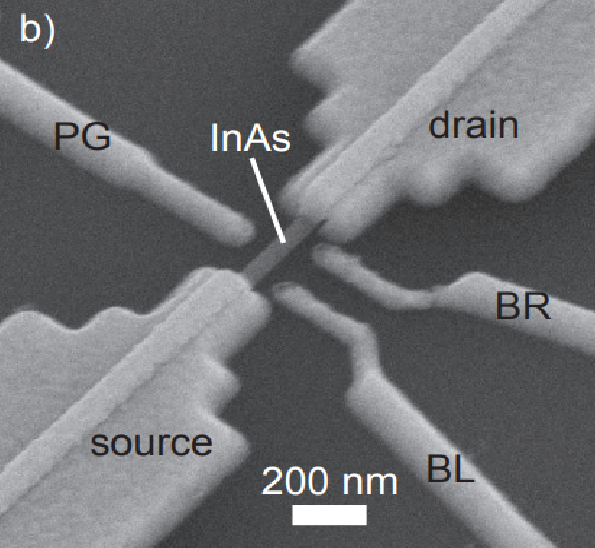
\includegraphics[width=.8\linewidth]{figures/qdotsem.png}
  \caption{}
  \label{fig:sem}
\end{subfigure}%
\begin{subfigure}[t]{.5\textwidth}
  \centering
  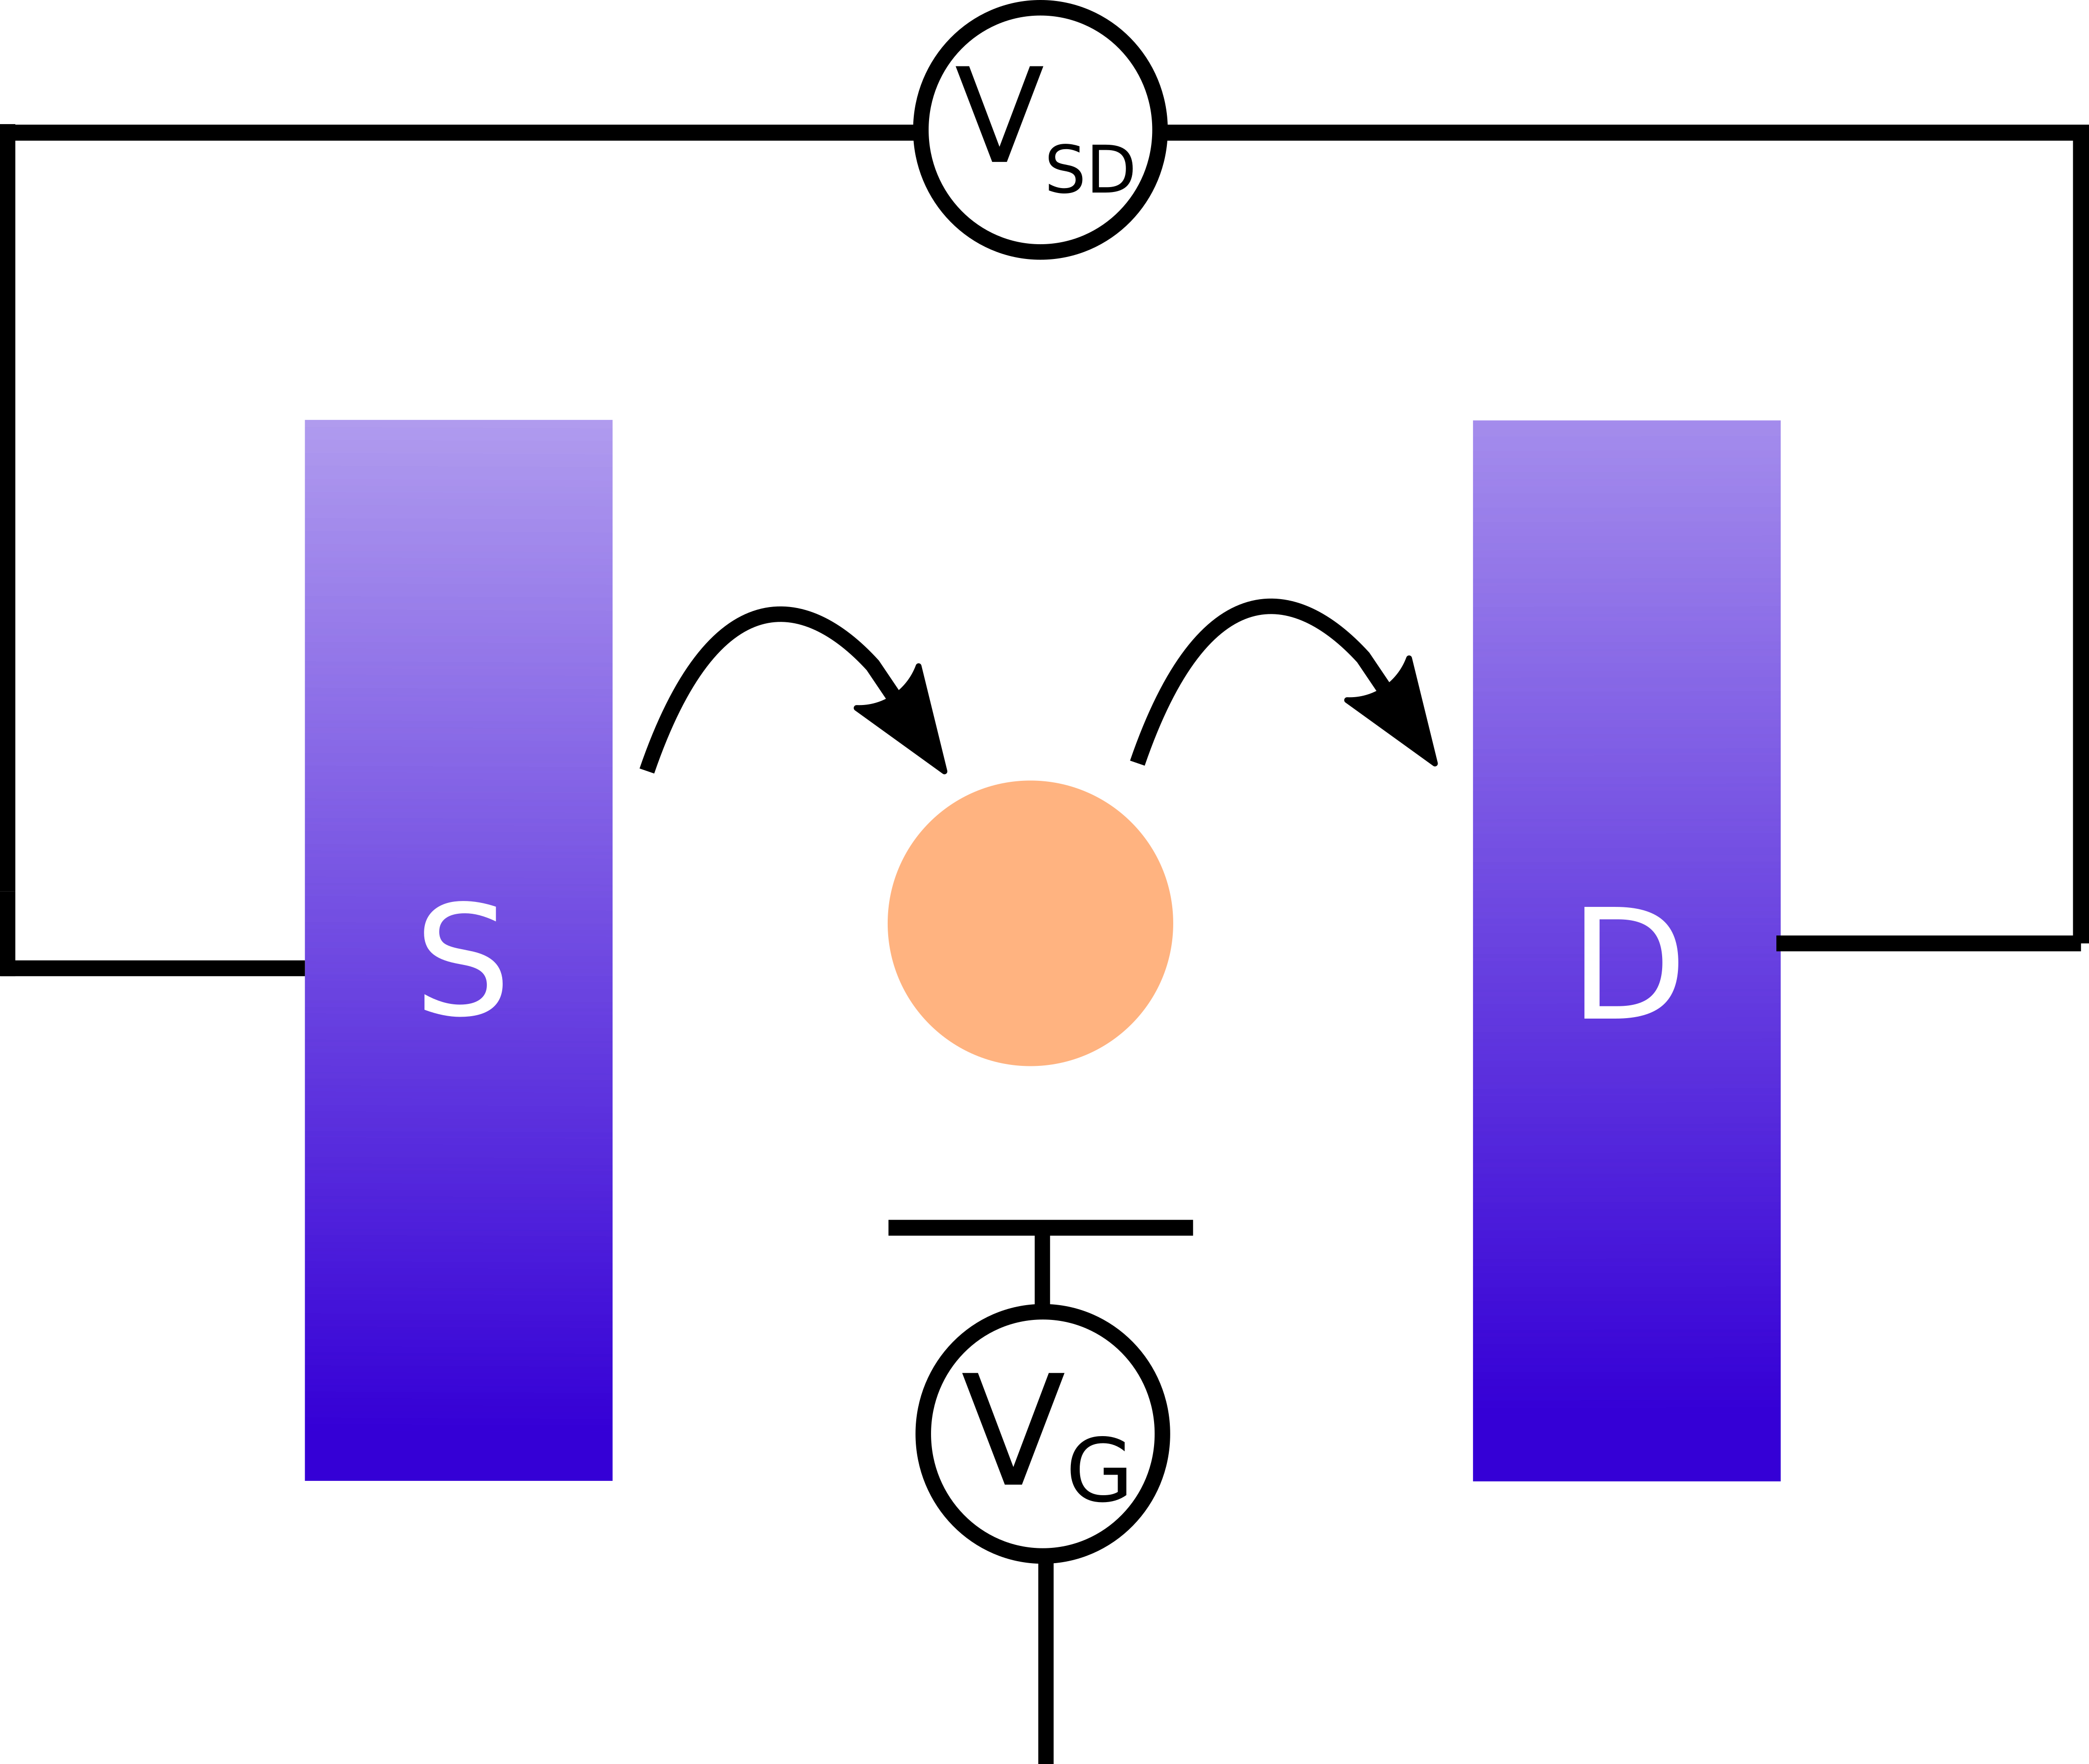
\includegraphics[width=.9\linewidth]{figures/qdotschematic.png}
  \caption{}
  \label{fig:qdotscheme}
\end{subfigure}
\caption{a) A physical implementation of a single QD system. The QD is realized within the InAs nanowire, with the source and drain, and the gates (BR, BL and PG) all clearly visible in this figure. The figure is taken from Ref.~\cite{sven}. b) A schematic figure of a QD system where the QD is in the center, tunnel coupled to the source (S) and drain (D). The gate voltage $V_\text{G}$ and the source-drain voltage $V_\text{SD}$, are tuned to define the QD.}
\label{fig:qdot}
\end{figure}

The wide tunability of the optical, electrical and chemical properties of QDs has made them useful in a large range of applications. Quantum dot technologies span areas from energy harvesting, display technologies, and sensors to medical and biological applications, with efficient lasers, biotags and solar harvesting devices being available on the market~\cite{qdotrev}. The transport set-up given in \cref{fig:qdot} in particular, is used as a very sensitive charge sensor, being able to detect transport of single electron charges, and single electron transistor (source). The QD systems studied in the literature have also included systems containing multiple QDs in various arrangements. In Ref.~\cite{doubledot}, a system with two QDs coupled in parallel was studied for its quantum interference effects in the transport dynamics, and was proposed to act as a sensitive electric switch.

In this thesis, the same parallel QD system was studied for its non-equilibrium transport properties, with focus on the full quantum dynamics, including the transient current. In particular, the dynamics at a second order EP is analyzed in detail using a combination of numerical and analytical approaches. Summarizing the results from the thesis, a second order EP was found, after which we derive and numerically implement the transient dynamics of the parallel dot system at and away from the EP. The evolution of the reduced density matrix in generalized modes is evidenced, including algebraic decay at the EP for certain initial conditions, as opposed to the exponential decay outside of the EP. Furthermore, the simulations of the current through the QDs indicated signatures of critical decay at the EP, similar to the study of quantum thermal machines in Ref.~\cite{thermal}.

% Inspired by Ref.~\cite{thermal} and its study of EPs in thermal machines, the main purpose of the thesis is to see if similar results are visible in QD systems. Considering the relative sparse amount of literature on EPs in Liouvillian physics, and especially in systems involving QDs, this ...


The thesis is divided in the following sections: in \cref{sec:theory} the underlying theory of the thesis is presented, including QD transport, open quantum systems and dynamics at EPs. \Cref{sec:sys} includes a further description of the parallel QD system and the model used to describe it. In \cref{sec:res} the results from the simulations are presented and in \cref{sec:disc}, the results are analyzed and an outlook is done.

\end{document}

